\documentclass[12pt,french]{book}
%___________________________
%===    Configurations 12.09.2013
%------------------------------------------------------
%packages permettant d'augmenter le nombre de registres de dimension et donc d'éviter les erreurs de compilation dûs aux packages tikz, pstricks and compagnie
\usepackage{etex}
%___________________________
%===    Pour le français
%------------------------------------------------------
\usepackage[utf8x]{inputenc}
\usepackage[T1]{fontenc}
\usepackage{babel}
\FrenchFootnotes

%___________________________
%===    Polices d'écriture
%------------------------------------------------------
%\usepackage{mathpazo}
\usepackage{frcursive} % Pour l'écriture cursive
\usepackage[upright]{fourier}% l'option permet d'avoir les majuscules droites dans les formules mathématiques
\usepackage[scaled=0.875]{helvet}

%___________________________
%===    Les couleurs
%------------------------------------------------------
\usepackage[dvipsnames,table]{xcolor}
%
\newcommand{\rouge}[1]{{\color{red} #1}}
\definecolor{midblue}{rgb}{0.145,0.490,0.882}
\newcommand\MaCouleur{midblue}

%___________________________
%===   Redéfinition des marges par défaut
%------------------------------------------------------
\setlength\paperheight{297mm}
\setlength\paperwidth{210mm}
\setlength{\evensidemargin}{0cm}% Marge gauche sur pages paires
\setlength{\oddsidemargin}{0cm}%{-0.5cm}% Marge gauche sur pages impaires
\setlength{\topmargin}{-2cm}% Marge en haut
\setlength{\headsep}{0.5cm}% Entre le haut de page et le texte
\setlength{\headheight}{0.7cm}% Haut de page
\setlength{\textheight}{25.2cm}% Hauteur de la zone de texte
\setlength{\textwidth}{17cm}% Largeur de la zone de texte

\usepackage{lscape} %permet le format paysage du document
\usepackage{xspace} % création automatique d'espaces dans les commandes
\setlength{\parindent}{0pt}

\usepackage{fancyhdr}
\pagestyle{fancy}
%
\renewcommand{\headrulewidth}{0pt}% pas de trait en entête
\newcommand\RegleEntete[1][0.4pt]{\renewcommand{\headrulewidth}{#1}}%commande pour ajouter un trait horizontal en entête

\newcommand{\entete}[3]{\lhead{#1} \chead{#2} \rhead{#3}}
\newcommand{\pieddepage}[3]{\lfoot{#1} \cfoot{#2} \rfoot{#3}}
%
%\renewcommand{\chaptermark}[1]{\markboth{#1}{}} % enregistre le titre courant du chapitre
    %en-tete droite page [paire] et {impaire}
%\rhead[]{\textbf{\leftmark.}}
    %en-tete gauche page [paire] et {impaire}
%\lhead[\textbf{\chaptername~\thechapter.}]{}


\usepackage{enumerate} %permet la modif de la numérotation et de poursuivre une numérotation en cours avec \begin{enumerate}[resume]
\usepackage{enumitem}
\frenchbsetup{StandardLists=true}%frenchb ne s'occupera pas des listes
\setenumerate[1]{font=\bfseries,label=\arabic*\degres)} % numérotation 1°) 2°) ...
%\setenumerate[2]{font=\itshape,label=(\alph*)} % sous-numérotation (a) (b) ...
\setenumerate[2]{font=\bfseries,label=(\alph*)} % sous-numérotation (a) (b) ...

\usepackage{lastpage} % permet d'afficher le nombre total de pages après DEUX compilations.

%___________________________
%===    Raccourcis classe
%------------------------------------------------------
\newcommand\seconde{2\up{nde}\xspace}
\newcommand\premiere{1\up{ère}\xspace}
\newcommand\terminale{T\up{le}\xspace}
\newcommand\stmg{\bsc{Stmg}}
\newcommand\sti{\bsc{Sti2d}}
\newcommand\bat{BAT 1\xspace}
\newcommand\BAT{BAT 2\xspace}
\newcommand\tesspe{TES Spécialité\xspace}


%___________________________
%===    Réglages et Commandes Maths
%------------------------------------------------------
%redéfinition de fractions, limites, sommes, intégrales, coefficients binomiaux en displaystyle, limites de suites
\usepackage{amssymb,mathtools}
\let\binomOld\binom
\renewcommand{\binom}{\displaystyle\binomOld}
\let\limOld\lim
\renewcommand{\lim}{\displaystyle\limOld}
\newcommand{\limn}{\lim_{n\to +\infty}} %limite lorsque n tend vers + infini
\newcommand{\limm}{\lim_{x\to -\infty}} %limite lorsque x tend vers - infini
\newcommand{\limp}{\lim_{x\to +\infty}} %limite lorsque x tend vers + infini
\newcommand{\limz}{\lim_{x\to 0}} %limite lorsque x tend vers 0
\newcommand{\limzm}{\lim_{\substack{x \to 0\\ x < 0}}} %limite lorsque x tend vers 0-
\newcommand{\limzp}{\lim_{\substack{x \to 0\\ x > 0}}} %limite lorsque x tend vers 0+
\let\sumOld\sum
\renewcommand{\sum}{\displaystyle\sumOld}
\let\intOld\int
\renewcommand{\int}{\displaystyle\intOld}

%\usepackage{yhmath}%permet les arcs de cercles
%\usepackage[euler-digits]{eulervm} %-> police maths
%
\usepackage{amssymb,mathtools}
\usepackage{stmaryrd}%\llbracket et \rrbracket % crochets doubles pour intervalles d'entier
%symbole parallèle avec \sslash

\newcommand{\crochets}[2]{\ensuremath{\llbracket #1 ; #2 \rrbracket}}

\newcommand{\intervalleff}[2]{\left[#1\,;#2\right]}
\newcommand{\intervallefo}[2]{\left[#1\,;#2\right[}
\newcommand{\intervalleof}[2]{\left]#1\,;#2\right]}
\newcommand{\intervalleoo}[2]{\left]#1\,;#2\right[}



\usepackage{bm} % pour l'écriture en gras des formules mathématiques avec \bm

\usepackage{cancel} % pour les simplifications de fractions
\renewcommand\CancelColor{\color{red}}
%\usepackage{siunitx} % écriture de nombres et d'unités
%\sisetup{output-decimal-marker={,},detect-all}
\usepackage[autolanguage,np]{numprint}
%permet les espacement pour les nombres décimaux avec \np{3,12456} en environnement maths ou pas
\DecimalMathComma %supprime l'espace après la virgule dans un nombre

%
\usepackage{dsfont} %écriture des ensemble N, R, C ...
\newcommand{\C}{\mathds C}
\newcommand{\R}{\mathds R}
\newcommand{\Q}{\mathds Q}
\newcommand{\D}{\mathds D}
\newcommand{\Z}{\mathds Z}
\newcommand{\N}{\mathds N}
\newcommand\Ind{\mathds 1} %= fonction indicatrice
\newcommand\p{\mathds P} %= probabilité
\newcommand\E{\mathds E} % Espérance
\newcommand\V{\mathds V} % Variance
\newcommand{\e}{\text{e}}
\newcommand{\dd}{\,\text{d}}

%Nombres complexes
\let\Reold\Re
\renewcommand{\Re}{~\text{Re}~}
\let\Imold\Im
\renewcommand{\Im}{~\text{Im}~}
\newcommand{\ii}{\,\text{i}}
% Exponentielle complexe
\newcommand{\ei}[2]{\,\e^{\dfrac{#1\ii\pi}{#2}}}


%
\usepackage{mathrsfs}   % Police de maths jolie caligraphie
\newcommand{\calig}[1]{\ensuremath{\mathscr{#1}}}
\newcommand\mtc[1]{\ensuremath{\mathcal{#1}}}


%Gestion des espaces
%
\newcommand{\pv}{\ensuremath{\: ; \,}}
\newlength{\EspacePV}
\setlength{\EspacePV}{1em plus 0.5em minus 0.5em}
\newcommand{\qq}{\hspace{\EspacePV} ; \hspace{\EspacePV}}
\newcommand{\qetq}{\hspace{\EspacePV} \text{et} \hspace{\EspacePV}}
\newcommand{\qouq}{\hspace{\EspacePV} \text{ou} \hspace{\EspacePV}}
\newcommand{\qLq}{\hspace{\EspacePV} \Leftarrow \hspace{\EspacePV}}
\newcommand{\qRq}{\hspace{\EspacePV} \Rightarrow \hspace{\EspacePV}}
\newcommand{\qLRq}{\hspace{\EspacePV} \Leftrightarrow \hspace{\EspacePV}}

%simplification notation norme \norme{}
\newcommand{\norme}[1]{\left\Vert #1\right\Vert}


%simplification de la notation de vecteur \vect{}
\newcommand{\vect}[1]{\mathchoice%
{\overrightarrow{\displaystyle\mathstrut#1\,\,}}%
{\overrightarrow{\textstyle\mathstrut#1\,\,}}%
{\overrightarrow{\scriptstyle\mathstrut#1\,\,}}%
{\overrightarrow{\scriptscriptstyle\mathstrut#1\,\,}}}



%Repères
\def\Oij{$\left(\text{O}\pv\vect{\imath},~\vect{\jmath}\right)$\xspace}
\def\Oijk{$\left(\text{O}\pv\vect{\imath},~ \vect{\jmath},~ \vect{k}\right)$\xspace}
\def\Ouv{$\left(\text{O}\pv\vect{u},~\vect{v}\right)$\xspace}
\def\OIJ{$\left(O\pv I\:,\,J\right)$\xspace}

\newcommand\abs[1]{\ensuremath{\left\vert #1 \right\vert}}%valeur absolue
\newcommand\Arc[1]{\ensuremath{\wideparen{#1}}}%arc de cercle


%symbole pour variable aléatoire qui suit une loi
\newcommand{\suit}{\hookrightarrow}

%___________________________
%===    Pour les tableaux
%------------------------------------------------------
\usepackage{array}
\usepackage{longtable}
\usepackage{tabularx,tabulary}
\usepackage{multirow}
\usepackage{multicol}
%exemple
%\begin{multicols}{3}[Titre sur une seule colonne.]
%   3~colonnes équilibrées, 3~colonnes équilibrées, 3~colonnes équilibrées, 3~colonnes équilibrées
%\end{multicols}
%\begin{multicols}{2}[\section{Titre numéroté.}]
%   blabla sur deux colonnes, c'est plus sérieux. C'est le style qui est généralement utilisé pour écrire des articles.
%saut de colonne forcé :
%\columnbreak
%djhskjdhjsq
%sdkksqjhd
%\end{multicols}
%Pour ajouter un titre numéroté qui apparaisse sur toute la largeur de la page, il faut utiliser l'option [\section{Titre.}] juste après \begin{multicols}{nb-col}.
%Remarques :
%Pour qu'une ligne de séparation apparaisse entre les colonnes, il faut utiliser : \setlength{\columnseprule}{1pt}.

%Pour redéfinir la largeur de l'espace inter-colonnes, il faut utiliser \setlength{\columnsep}{30pt}.

%Pour remonter le texte, dans chaque colonne vers le haut : \raggedcolumns qui se tape :\begin{multicols}{2}\raggedcolumns...\columnbreak...\columnbreak\end{multicols}

%Pour supprimer les traits verticaux : \setlength{\columnseprule}{0pt} avant \begin{multicols}{3}...\end{multicols}
\setlength\columnseprule{0.4pt}
\renewcommand{\arraystretch}{1.5}%augmente la hauteur des lignes des tableaux
%colonnes centrées verticalement et horizontalement permettant d'écrire des paragraphes de largeur fixée du type M{3cm}
\newcolumntype{M}[1]{>{\centering\arraybackslash}m{#1}}%cellule centrée horizontalement et verticalement
%\arraybackslash permet de continuer à utiliser \\ pour le changement de ligne

\usepackage{arydshln}% permet des filets horizontaux ou verticaux en pointillés avec
%pour les filets horizontaux \hdashline ou \cdashline qui s'utilisent comme \hline ou \cline
% pour les filets verticaux les deux points :


%___________________________
%===    Divers packages
%------------------------------------------------------
\usepackage{bclogo}
\usepackage{textcomp}
\usepackage{eurosym}%avec \EUR{3,12}
\usepackage{soul} % Pour souligner : \ul
\usepackage{ulem} % Pour souligner double : \uuline
                      % Pour souligner ondulé : \uwave
                      % Pour barrer horizontal : \sout
                      % Pour barrer diagonal : \xout
\usepackage{tikz,tkz-tab,tkz-graph}
\usetikzlibrary{calc,shapes,arrows,plotmarks,lindenmayersystems,decorations,decorations.pathreplacing,patterns}
\usepackage{pstricks,pst-plot,pst-text,pstricks-add,pst-eucl,pst-all}


%INTERLIGNES
\usepackage{setspace}
%s'utilise avec \begin{spacing}{''facteur''}
%   […]
%\end{spacing}

%Pointillés sur toute la ligne
\usepackage{multido}
\newcommand{\Pointilles}[1][1]{%
\multido{}{#1}{\makebox[\textwidth]{\dotfill}\\[1.5\parskip]
}}
%commandes : \Pointilles ou \Pointilles[4] pour 4 lignes


%textes à trous
\newlength\lgtrou
\newcommand*\trou[1]{%
\settowidth\lgtrou{#1}%
\makebox[2\lgtrou]{\dotfill}
\setlength\baselineskip{1.2\baselineskip}}
%Commande à utiliser : \trou{texte qui sera remplacé par des pointillés}

%divers cadres
\usepackage{fancybox} % par exemple \ovalbox{}

%caractères spéciaux avec la commande \ding{230} par exemple
\usepackage{pifont}

%___________________________
%===    Quelques raccourcis perso
%------------------------------------------------------
\newcommand\pfr[1]{\psframebox[linecolor=red]{#1}}
\newcommand\coef[1][]{c{\oe}fficient#1\xspace}


%QRcode, codebarre
\usepackage{pst-barcode}
%\begin{pspicture}(2,2)
%	\psbarcode{http://www.latex-howto.be}{eclevel=M}{qrcode}
%\end{pspicture}


%Texte en filigrane
\usepackage{watermark}
%On utilise ensuite les commandes \watermark, \leftwatermark, \rightwatermark ou \thiswatermark qui permettent de définir un filigrane sur toutes les pages, les pages paires, les pages impaires ou juste une page
%Exemple : \thiswatermark {
%\begin{minipage}{0.95\linewidth}
%\vspace{25cm}
%\begin{center}
%\rotatebox{55}{\scalebox{8}{\color[gray]{0.7}\LaTeX}}
%\end{center}
%\end{minipage}
%}

%QCM
\usepackage{alterqcm}					%%Permet de créer des QCM
%\begin{alterqcm}
%\AQquestion{Question}{{Proposition 1},{Proposition 2},{Proposition 3}}
%\end{alterqcm}

%\dingsquare %carré avant V ou F
%\dingchecksquare %carré validé devant V ou F


%Rond entourant une lettre avec pour arguments la couleur de fond, puis la lettre
\newcommand\rond[2][red!20]{\tikz[baseline]{\node[fill=#1,anchor=base,circle]{\bf #2};}}


%Ecrire card en écriture normale :
\newcommand{\card}{\text{card}\xspace}


%___________________________
%===    ALGORITHMES
%------------------------------------------------------

%ALGORITHME avec Algobox
\usepackage{ucs}
\usepackage{framed}
\definecolor{fond}{gray}{0.95}
\newenvironment{cadrecode}{%
  \def\FrameCommand{{\color[HTML]{888888}\vrule width 3pt}\colorbox{fond}}%
  \MakeFramed {\advance\hsize-\width \FrameRestore}}%
{\endMakeFramed}
\usepackage{alltt}

% Mise en forme des algorithmes
\usepackage[french,boxed,titlenumbered,lined,longend]{algorithm2e}
  \SetKwIF {Si}{SinonSi}{Sinon}{si}{alors}{sinon\_si}{alors}{fin~si}
 \SetKwFor{Tq}{tant\_que~}{~faire~}{fin~tant\_que}
 \SetKwFor{PourCh}{pour\_chaque }{ faire }{fin pour\_chaque}
 \SetKwInput{Sortie}{Sortie}
  \SetKwInput{Entree}{Entrée}
\newcommand{\Algocmd}[1]{\textsf{\textsc{\textbf{#1}}}}\SetKwSty{Algocmd}
  \newcommand{\AlgCommentaire}[1]{\textsl{\small  #1}}


%___________________________
%===    MISE EN FORME EXERCICES
%------------------------------------------------------
%\usepackage{marvosym}
\usepackage{slashbox}

\newcounter{exo}
\newenvironment{exo}{%
  \refstepcounter{exo}\Writinghand\ \textbf{Exercice \theexo.}\par
  \medskip}%
{\[*\]}


%___________________________
%===    HYPERLIENS
%------------------------------------------------------
\usepackage[colorlinks=true,linkcolor=black,filecolor=blue,urlcolor=blue,bookmarksnumbered]{hyperref} 


\renewenvironment{exo}[1]{%
  \refstepcounter{exo}\underline{\textbf{Exercice \theexo :}} \quad \textit{#1}\par
  \medskip}%
{\bigskip}

\pieddepage{}{}{\thepage}

\begin{document}
\underline{\textbf{\bsc{Contrôle commun de seconde}}} \hspace{\stretch{1}} \underline{\textbf{\bsc{Nom} :}} \hspace{\stretch{2}} \underline{\textbf{Classe :}} \hspace{\stretch{2}}\medskip

{\sffamily
Jeudi $28$ février $\np{2013}$ - \textbf{Durée :} 2 heures - 4 \textbf{exercices à traiter} - Le sujet comporte \pageref{LastPage} pages - \medskip

\textbf{Rendre le sujet avec la copie.} Le barème est indicatif.
}\bigskip

\begin{exo}{($9,5$ points)}
    Soit \Oij un repère orthonormé du plan.\par 
    Soient les points $A(-5 \pv -4)$, $B(-1 \pv 6)$ et $C(1 \pv 2)$.

    \begin{enumerate}
        \item Faire une figure que l'on complétera au fur et à mesure de l'exercice.
        \item Montrer que le triangle $ABC$ est rectangle isocèle.
        \item Calculer les coordonnées du milieu $\Omega$ du segment $[AC]$.
        \item Déterminer le \coef directeur de la droite $(AB)$.
        \item Déterminer une équation de la droite $\Delta$ parallèle à la droite $(AB)$ passant par le point $C$.
        \item Calculer les coordonnées du point d'intersection $D$ de la droite $\Delta$ et de l'axe des abscisses.
        \item \begin{enumerate}
                        \item Tracer la droite $d$ d'équation $y = -2 x - 6$.
                        \item Le point $D$, défini à la question 6, appartient-il à la droite $d$ ?
                \end{enumerate}
        \item Déterminer la nature du quadrilatère $ABCD$. Justifier soigneusement la réponse.
    \end{enumerate}
\end{exo}

\begin{exo}{($8,5$ points)}
    Une usine fabrique des rouleaux de tissu qu’elle vend à des ateliers de confection.\par
    Le fournisseur veut contrôler la conformité de sa production. Pour cela il prend un échantillon de $200$ rouleaux et mesure les longueurs de tissu de ceux-ci. Toutes les mesures de longueurs sont exprimées en mètres. Il obtient les résultats suivants :

    \begin{center}
    \scriptsize    
        \begin{tabular}{|>\bfseries c|*{14}{c|}}
          \hline
            Longueur & $49,4$ & $49,5$ & $49,6$ & $49,7$ & $49,8$ & $49,9$ & $50,0$ & $50,1$ & $50,2$ & $50,3$ & $50,4$ & $50,5$ & $50,6$ & $50,7$ \\
          \hline
            Effectif & $2$ & $8$ & $4$  & $19$  & $25$  & $29$  & $33$  & $30$  & $22$  & $15$  & $7$  & $3$  & $2$  & $1$  \\
          \hline
            E.C.C. &   &   &   &   &   &   &   &   &   &   &   &   &   &   \\
          \hline
        \end{tabular}
    \end{center}

    \begin{enumerate}
        \item Compléter la ligne ECC (effectifs cumulés croissants) dans le tableau ci-dessus.
        \item Déterminer la valeur exacte puis la valeur arrondie à $0,01$ près de la moyenne de cette série. Interpréter cette valeur dans le cas étudié.
        \item Déterminer la médiane $M_e$ de cette série. Justifier votre calcul.
        \item Déterminer les quartiles $Q_1$ et $Q_3$ de cette série. Justifier vos résultats.
        \item Préciser l’étendue de cette série.
    \end{enumerate}
    
Le fournisseur a alors établi un protocole de conformité : pour qu’un rouleau de tissu soit conforme, la longueur de tissu doit appartenir à l’intervalle $\intervalleff{49,6}{50,4}$.

    \begin{enumerate}[resume]
        \item Calculer le pourcentage de rouleaux conformes de cet échantillon.
        \item De plus il estime que la machine nécessite un réglage si, dans un échantillon de $200$ rouleaux,  le pourcentage de rouleaux non conformes est strictement supérieur à $10\%$.\par Est-ce le cas ?
    \end{enumerate}
\end{exo}

\clearpage % force le changement de page

\entete{}{\underline{\textbf{\bsc{Nom} :}}}{\underline{\textbf{Classe :}}\hspace{2cm}}

\begin{exo}{(13 points)}
    \underline{\textbf{Partie A :}}\medskip
    
    Soit $f$ la fonction définie sur $\R$ par $f(x) = 0,1x^2 + 2x + \np{1000}$.\medskip
    
    \begin{enumerate}
        \item Calculer l'image de $100$ par $f$.\label{image}
        \item Vérifier que, pour tout $x \in \R$, $0,1x^2 + 2x - \np{2550} = (0,1x + 17)(x - 150)$.
        \item Résoudre dans $\R$ l'équation $0,1x^2 + 2x - \np{2550} = 0$.
        \item En déduire, par le calcul, les éventuels antécédents de $\np{3550}$ par $f$.\label{antecedent}
    \end{enumerate}\medskip
    
    \underline{\textbf{Partie B :}}\medskip

    \begin{minipage}{0.5\textwidth}
        Une entreprise produit et commercialise des tables.\par
        Le coût de production de $x$ tables est donné par la formule : $C(x) = 0,1x^2 + 2x + \np{1000}.$

        La courbe de la fonction $C$ est représentée sur $\intervallefo{0}{+\infty}$ dans le repère ci-contre.

        \begin{enumerate}
            \item Déduire des réponses aux questions \ref{image} et \ref{antecedent} de la partie A des informations concrètes sur la fonction coût $C$.
            \item Chaque table est vendue \EUR{$27$}. Ainsi, la recette $R(x)$ réalisée par l'entreprise correspondant à $x$ tables vendues est \[R(x) = 27x.\]
            \begin{enumerate}
                \item De quel type de fonctions s'agit-il ?
                \item De quelle nature est la représentation graphique de la fonction $R$ ?
                \item Tracer la coure représentative de $R$ sur le même graphique que la courbe de $C$.
            \end{enumerate}
            \item On appelle "bénéfice" la différence entre la recette et le coût de production.
            Ainsi, le bénéfice $B(x)$ pour $x$ tables produites et vendues est $B(x) = R(x) - C(x)$.\par\medskip
            Déterminer graphiquement le nombre de tables que l'entreprise doit produire et vendre pour réaliser un bénéfice strictement positif.
        \end{enumerate}
    \end{minipage}\qquad
    \begin{minipage}{0.4\textwidth}
        \begin{center}
            \begin{tikzpicture}[xscale=0.02,yscale=0.35]
                \draw[style=help lines] (-25,-1) grid[xstep=50,ystep=1] (225,40);
                \draw[->] (-25,0) -- (225,0);
                \draw[->] (0,-1) -- (0,41.5);
                \draw[blue,thick,domain=0:215,samples=200]plot(\x,{(0.1*\x*\x+2*\x+1000)/150});
                \foreach \x in {0,50,...,200} \draw(\x,0) node {\tiny$\vert$} node[below right=-3.5pt] {\tiny $\x$};
                \foreach \x in {-150,0,...,6000} \draw(0,\x/150) node {$-$} node[left] {\tiny$\x$};
            \end{tikzpicture}
        \end{center}
    \end{minipage}

\medskip

    \underline{\textbf{Partie C :}}\medskip
    
    \begin{enumerate}
        \item Vérifier que, pour tout $x \in \R$, $B(x) = -0,1x^2 + 25x - \np{1000}$.
        \item À l'aide de la calculatrice, remplir de tableau de valeurs ci-dessous :
            \[\begin{array}{|c|*{10}{>{\centering\arraybackslash}p{1cm}|}}
                \hline
                    x & 0 & 20 & 50 & 80 & 100 & 125 & 150 & 170 & 200 & 230 \\
                \hline
                    B(x) & & & & & & & & & & \\
                \hline
            \end{array}\]
            
        \item Tracer la courbe représentative de la fonction $B$ dans le repère ci-dessous :
        
            \begin{tikzpicture}[xscale=0.06,yscale=0.1]
                \draw[style=help lines] (-15,-55) grid[xstep=10,ystep=5] (239,60);
                \draw[->] (-12,0) -- (240,0);
                \draw[->] (0,-57) -- (0,63);
                \foreach \x in {10,20,...,230} \draw(\x,0) node {\tiny$\vert$} node[below] {\tiny $\x$};
                \draw (-10,0) node {\tiny$\vert$} node[below left=-3] {\tiny $-10$};
                \draw (0,0) node[below right=-3pt] {\tiny $0$} node[above left=-3.5pt] {\tiny $0$};
                \foreach \x in {-550,-500,...,-50} \draw(0,\x/10) node {$-$} node[left] {\tiny$\x$};
                \foreach \x in {50,100,...,600} \draw(0,\x/10) node {$-$} node[left] {\tiny$\x$};
            \end{tikzpicture}
        
        \item Donner le tableau de variations de la fonction $B$ sur $\intervalleff{0}{230}$.
        
        \item Quel doit être le nombre de tables produites et vendues par l'entreprise pour qu'elle réalise le bénéfice maximal ? Quel est ce bénéfice maximal ?
    \end{enumerate}
\end{exo}

\clearpage

\begin{exo}{($10,5$ points)}
    Le tableau donné en Annexe 1 fournit pour $\np{2012}$ la répartition des accidents corporels de la route par tranche horaire de la journée.
    
    \begin{enumerate}
        \item Déterminer la fréquence en pourcentage arrondie au dixième et la fréquence cumulée croissante de chacune des classes. On reportera les valeurs sur le tableau donné en Annexe 1.
        \item Compléter le polygone des fréquences cumulées croissantes dans le repère de l'Annexe 1.
        \item
            \begin{enumerate}
                \item Déterminer graphiquement une valeur approchée de la médiane $M_e$ et des premier et troisième quartiles $\mtc Q_1$ et $\mtc Q_3$. Les résultats seront donnés en heures minutes et on laissera les pointillés apparents.
                \item Interpréter le premier quartile.
            \end{enumerate}
        \item
            \begin{enumerate}
                \item L'affirmation << $50\%$ des accidents corporels ont lieu avant midi >> est-elle vraie ou fausse ? Justifier.
                \item L'affirmation << au moins $50\%$ des accidents corporels ont lieu entre $10$h et $19$h >> est-elle vraie ou fausse ? Justifier.
                \item À partir de quelle heure peut-on dire que $80\%$ des accidents corporels ont eu lieu dans la journée ?
            \end{enumerate}
    \end{enumerate}
\end{exo}

\clearpage

\begin{center}
    \underline{\textbf{Annexe 1}}
\end{center}\bigskip

\begin{center}
    \begin{tabularx}{0.75\textwidth}{|c|>\centering X|>\centering X|>{\centering\arraybackslash} X|}
        \hline
            \rowcolor{gray!50} Heure & Accidents corporels & Fréquence & FCC \\
        \hline
            $\intervallefo{0}{3}$ & $\np{3800}$ & & \\
        \hline
            $\intervallefo{3}{6}$ & $\np{2000}$ & & \\
        \hline
            $\intervallefo{6}{9}$ & $\np{10330}$ & & \\
        \hline
            $\intervallefo{9}{12}$ & $\np{12070}$ & & \\
        \hline
            $\intervallefo{12}{15}$ & $\np{16050}$ & & \\
        \hline
            $\intervallefo{15}{18}$ & $\np{19600}$ & & \\
        \hline
            $\intervallefo{18}{21}$ & $\np{18000}$ & & \\
        \hline
            $\intervallefo{21}{24}$ & $\np{8150}$ & & \\
        \hline
            Total & $\np{90000}$ & & \multicolumn{1}{c}{}\\
        \cline{1-3}
    \end{tabularx}
\end{center}\vfill

\begin{tikzpicture}[xscale=0.6,yscale=0.12]
    \draw[style=help lines] (0,0) grid[xstep=0.5,ystep=2] (25.5,105);
    \draw[->] (0,0) -- (25.5,0);
    \draw[->] (0,0) -- (0,105);
    \foreach \x in {0,1,...,25} \draw(\x,0) node {\tiny$\vert$} node[below] {\tiny$\x$};
    \foreach \x in {5,10,...,100} \draw(0,\x) node {\tiny$-$} node[left] {\tiny$\x$};
    \draw[color=OliveGreen,line width=1pt] plot[mark=o,mark size=5pt] coordinates {(0,0) (3,4.22)};
    % La marque est ici écrasée à cause de l'échelle des ordonnées.
    % Autres types de marque : asterisk, -,|, star, oplus, diamond, square, otimes, triangle, pentagon.
    % une alternative à la place est d'utiliser la ligne suivante :
    %\draw (0,0) node{\tiny$\bullet$} -- (3,4.22) node{\tiny$\bullet$};
\end{tikzpicture}
\end{document}